\documentclass[a4paper,10pt]{article}
\usepackage[utf8]{inputenc}
\usepackage[russian]{babel}
\usepackage{amsmath}
\usepackage{amssymb}

\DeclareMathOperator{\rot}{rot}
\DeclareMathOperator{\mdiv}{div}
\DeclareMathOperator{\RE}{Re}
\renewcommand{\Re}{\mathop{\mathrm{Re}}\nolimits}

%opening
\title{Моделирование отражения радиоволн от сложных полигональных моделей}
\author{Ефремов Андрей Сергеевич}
\date{xx.xx.xxxx} 

\begin{document}

\maketitle

\begin{abstract}
  aaaaaaa
\end{abstract}


  \newpage
\section*{Введение}

При использовании радиолокации интересной является задача моделирования распространения электромагнитного сигнала и определение зон, затемененных объектом, а также областей, распространения переотраженного сигнала. Особенно это важно при использовании радиотехнических систем на протяженных объектах, так как возникают дополнительные ошибки измерения радиолокационных параметров, например, при стыковках космических кораблей и работе космических станций. [*Сазонов]. 

Однако, при попытках детального моделирования описанного выше процесса, мы неминуемо приходим к тому, что используемые компьютерные модели космических объектов обладают огромным количеством полигонов, а вычислительных ресурсов даже современных персональных компьютеров не хватает для их обработки. 

Проведем простые предварительные расчеты. Если наша модель содержит 10 000 полигонов, то для того, чтобы  определить, какие грани являются первичными для всей модели нам потребуется обработать порядка $ 10^8 $ полигонов (без алгоритмических оптимизаций, "влоб"). Мы же в работе будем использовать модель космического корабля "Союз" [*wiki], содержащий 152 000 полигонов. Это число внушительно, просто необходимы большие мощности. Поэтому для расчетов будем использовать вычисления на графических ускорителях и технологию CUDA. 

Графические ускорители выросли из задач обработки и формирования изображения на экране компьютера постепенно переродившись в массивно-параллельные процессоры общего назначения. Сам термин GPU (Graphics Processing Unit) относительно новый и впервые был использован корпорацией Nvidia, в качестве обозначения того, что графические ускорители стали мощными программируемыми устройствами пригодными для решения более широкого класса задач, не связанных с графикой. [*боресков основы работы с cuda]

Первые графические ускорители представляли из себя простые растеризаторы, однако эту простую задачу делали быстрее универсального процессора, что и привело к распространению графических ускорителей. Основная причина этого -- ускоритель мог обрабатывать хоть и простую, но зато масштабную работу -- обрабатывать сразу много отдельных пикселов. [*боресков]

По мере развития функциональность увеличивалась. Фактически графические ускорители стали представлять из себя SIMD-процессоры (Single Instruction Multiple Data), то есть параллельные устройства, способные одновременно выполнять одну и ту же операцию над многими данными. Экспоненциальный рост производительности и функциональности дал развитие направлению GPGPU (General-Purpose computing on Graphics Processing Units). 

Все это открывает новые возможности при реализации приложений, требущих больших объемов специфических вычислений. И если раньше ресурсоемкие задачи и можно было решить, то только с использованием суперкомпьютеров и кластеров, то теперь это представляется возможным на обычном пользовательском  компьютере. 

На сегодняшний день существуют несколько технологий для разработки приложений, использующих для вычислений графические ускорители: OpenCL, CUDA, ATI Stream Technology. В нашей работе мы остановимся на технологии Nvidia CUDA и будем использовать её. 

Тому причин несколько. Nvidia CUDA хорошо зарекомендовала себя при решении многих ресурсоемких задач: моделирование гидродинамики [*березин], волн цунами [*курако], ускорение вычисления нейронных сетей [*парубец].



  \newpage
\section*{Модели отражения} 

Радиоволна, как и любая другая электромагнитная волна, отражается от препятствий, причем препятствием является любая неоднородность электрических или магнитных параметров среды, то есть объект отражает электромагнитную энергию, в случае если проводимость, диэлектрическая или магнитная проницаемость отличается от соответствующих параметров среды.
Так как от поверхности в результате процесса отражения отходит электромагнитная энергия, то можно считать, что отражатель сам является источником (вторичным) электромагнитного излучения. Это явление можно также представить себе следующим образом: при попадании волны на поверхность предмета, она в нем порождает вынужденные колебания зарядов, которые синхронны с колебаниями падающей волны. Колебания зарядов создают токи смещения и токи проводимости, и сами становятся источниками излучения. Каждый такой элементарный ток в рамках достаточного малого точечного объема можно считать источником новой сферической волны. Общий результат таких элементарных токов (в соответствии с принципом Гюйгенса-Френеля \cite{gugens}) суммируется с различными фазовыми соотношениями и может принимать разные значения, а падающая волна отражается во всех направлениях. Значит, энергия переизлучается в различных направлениях неравномерно \cite{radiolocation}.

Радиоволны и световые волны имеют одну и ту же физическую электромагнитную природу, поэтому многие модели поведения света известные из оптики (кстати как и способы получения фотореалистических изображений компьютерной геометрии) применимы в нашем случае. Рассмотрим основные модели отражения радиоволн: зеркальное, диффузное и резонансное. Подробнее информацию об этом можно найти в \cite{radiolocation}.

\subsection*{Зеркальное отражение}

Условие возникновения: линейные размеры отражающей поверхности много больше длины волны ($ l >> \lambda $), а сама поверхность является достаточно гладкой ($ h << \lambda $), где $ l $ -- наименьшией линейный размер цели; $ \lambda $ -- длина волны; $ h $ -- высота неровностей поверхности. 

Свойства зеркального отражения известны еще с давних времен и являются следствиями применения принципа Ферма к отражающей поверхности \cite{ferma}:

- луч отраженный, луч падающей, а также нормаль отражающей поверхности, проведенная к точке падения, лежат в одной плоскости;

- угол падения равен углу отражения.

\begin{center}
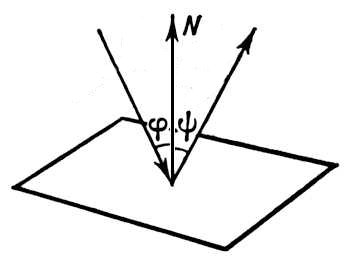
\includegraphics[width=0.25\linewidth]{zerkalo.jpg}
\end{center}

Интенсивность отражённого света характеризуется коэффициентом отражения и зависит от соотношения показателей преломления сред, от угла падения и поляризации падающего пучка лучей. Количественно эту зависимость выражают формулы Френеля \cite{frenel}.

\subsection*{Диффузное отражение}

Условие возникновения: линейные размеры отражающей поверхности много больше длины волны ($ l >> \lambda $), а неровности поверхности имеют порядок длины волны (или больше) и расположены хаотично, то есть поверхность является шераховатой (матовой) ($ h \ge \lambda $). 

При диффузном отражении энергия рассеивается во всех направлениях. Для матовых поверхностей применимы законы Ламберта \cite{lambert}: для потока излучения, падающего нормально к матовой поверхности, мощность вторичного излучения под углом $ \gamma $ к нормали пропорциональна $ cos \gamma $. 
\begin{gather}
 P = P_0 \cdot cos \gamma
\end {gather}

\begin{center}
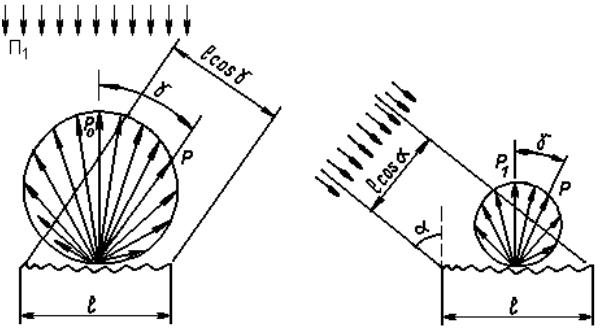
\includegraphics[width=0.6\linewidth]{lambert.jpg}
\end{center}

Если поток излучения падает под углом $\alpha$ к поверхности, то 
\begin{gather}
 P = P_0 \cdot cos \alpha \cdot cos \gamma
\end {gather}
где $ P_0 $ -- мощность, которую принимал бы приемник, если бы облучение шло с "зенита", то есть с увеличением $\alpha$ уменьшается перехватываемый поверхностью падающий поток, отчего уменьшается освещенность и яркость. 

Условия зеркальности и диффузно отражающих поверхностей являются расплывчатыми. Здесь \cite{radiolocation} дается строгая формулировка и вывод критерия различия зеркальных и матовых поверхностей. Скажем лишь, что тип поверхностей зависит сразу от трех факторов: высоты неровностей поверхности $h$, длины волны $\lambda$ и угла падения $\phi$.

Закон Ламберта -- закон идеального рассеивания света, то есть это некоторая модель, к которой можно приблизиться, но которой не существует в естественных условиях. В реальной жизни поверхности обычно дают отражение, представляемое смесью диффузной и зеркальной состовляющих. 

\begin{center}
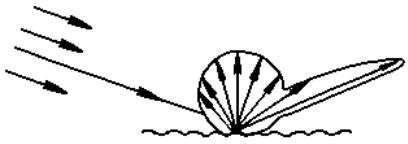
\includegraphics[width=0.45\linewidth]{diffuzerkalo.jpg}
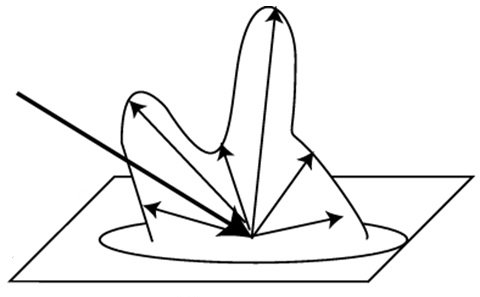
\includegraphics[width=0.45\linewidth]{glossy.jpg}
\end{center}

Кроме того, на практике, часто встречаются материалы имеющие несколько максимумов под разными углами и дающие в соответствующих направлениях из-за этого блеск (glossy materials).

Все вышеперечисленные свойства можно смоделировать воспользовавшись функцией, характеризующей степень отражения в данном направлении. Такая функция называется ДФО -- двулучевая функцией отражения (BRDF -- Bidirectional Reflection Distribution Function). Так для диффузных моделей ДФО равна константе. 

\begin{center}
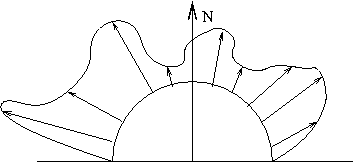
\includegraphics[width=0.45\linewidth]{dfo.png}
\end{center}

Именно эту функцию мы и будем использовать в нашей работе. Таким образом достигается некоторая универсальность -- наша программа сможет моделировать не только какой-то один конкретный вид отражения, а появляется возможность это задать в достаточно независимом виде. 

\subsection*{Резонансное отражение}

Список моделей отражения был бы не полон если не упомянуть резонансное отражение. Как уже было отмечено, падающая волна создает вынужденные колебания свободных или связанных зарядов в поверхности предмета. Тело, способное переизлучать электромагнитную волну, обладает собственной частотой колебаний частиц, несущих электрический заряд. Причем, если частота колебаний падающей волны совпадает с собственной частотой колебаний в поверхности, то имеем не что иное как явление резонансного отражения. В этом случае появляется ярко выраженная направленность вторичного излучения. Подробнее об этом явлении можно прочитать в \cite{radiolocation}.



  \newpage
\section*{Математическая постановка задачи}

Предположим, у нас есть ненаправленная антенна, представляемая точечным источником (расстояние до поверхности значительно больше размеров антенны) с излучающей мощностью $P_0$. Тогда вся энергия распределяется равномерно по всей поверхности некоторой сферы радиуса $R$, площадь поверхности которой равна $ 4 \pi R^2 $. Таким образом, источник электромагнитного излучения создает плотность потока мощности
\begin{gather}
   J = \frac{P_0}{4 \pi R^2}
\end{gather}
Следовательно, каждая точка поверхности $ M(x, y, z) $, которая располагается в зоне прямой видимости, получает от источника излучения в секунду энергию мощности на единицу площади равную
\begin{gather}
  dP_{in} =   \left\langle  {\vec{J}(x,y,z) \cdot  \vec{d\sigma} } \right\rangle = J(x,y,z) \cdot d\sigma \cdot cos \phi ,
\end{gather}
где $d\sigma$ -- окрестность точки $ M(x, y, z) $, а $\phi$ -- угол между вектором $ \vec{J}(M) $ и нормалью к поверхности $d\sigma$, направленной в противоположную сторону от источника излучения.  

Значит, учитывая $(4)$, первично-освещенная поверхность получает в секунду энергию мощности, равную 
\begin{gather}
  P_{in} =   \int \limits_S \left\langle  {\vec{J}(x,y,z) \cdot  \vec{d\sigma} } \right\rangle,
\end{gather}
где $ S $ -- первично-освещенная поверхность.

Часть энергии попадаемые в точки первично-освещенных поверхностей поглощается, часть отражается. Точки, отражающие электромагнитные волны ведут себя как вторичные источники электромагнитного излучения, а значит вышепроделанные умозаключения к ним тоже применимы. 

После многократного отражения и переотражения получаем, что для каждой точки $ M(x,y,z) $ справедливо
\begin{gather}
  J_{out}(x,y,z,\vec \omega) = \int \limits_\Omega J_{in}(x,y,z,\vec \theta) \cdot f(x,y,z,\vec \omega,\vec \theta) \cdot \left\langle  {-\vec \theta \cdot \vec n} \right\rangle \cdot d\theta,
\end{gather}

где $ J_{out} $ -- поток из точки $(x,y,z)$ в направлении вектора $ \vec \omega $, а $ J_{in} $ -- поток входящего в точку $(x,y,z)$ излучения из направления вектора $ \vec \theta $. В данном уравнении интеграл взят по $ \Omega $ -- совокупности входящих направлений в точку $M(x,y,z)$, $\theta$ -- телесный угол, порожденный вектором $\vec \theta$. Способ отражения от поверхности, а также соотношение отраженной энергии и поглощенной задано в общем случае двулучевой функцией отражения $ f(x,y,z,\vec \omega,\vec \theta) $. 

\begin{center}
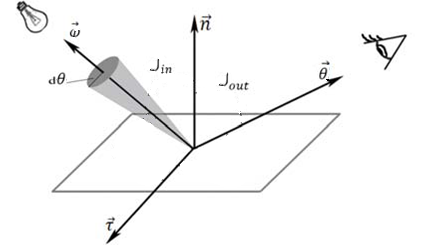
\includegraphics[width=0.499\linewidth]{rendering-equation.png}
\end{center}

Уравнение $(6)$ является частным случаем более общего уравнения, называемого уравнением рендеринга  \cite{rendering-equ}. Существует несколько подходов к его решению. Рассмотрим их.

  \section*{Реализация}

1. ------------Трассировка лучей --------------

Для определения видимости полигона $ \alpha $ из точки $ L $, рассматривается отрезок $ LP $, где $ P $ -- центр полигона. Находятся все пересечения отрезка с полигонами модели (разумеется, многоугольник $ \alpha $ не подлежит рассмотрению). Если таких граней не нашлось, то грань $ \alpha $ считается видимой из точки $ L $, иначе -- невидимой. 

Задача определения пересечения отрезка и многоугольника разбивается на следующие этапы.

1. Определить точку пересечения $ M $ плоскости многоугольника и прямой, содержащей отрезок.

2. Находится ли точка пересечения $ M $ внутри многоугольника.

3. Находится ли точка пересечения $ M $ внутри отрезка.

Несмотря на то, что для достаточно детализированной модели с количеством полигонов в несколько тысяч, данный процесс достаточно трудоемок, в работе программе исходной статьи никакие способы оптимизации не использовались. Способов оптимизации действительно много и сравнение самых популярных можно прочитать в [*].


  \newpage
\section*{Результаты} 

Результатом работы стало программное обеспечение, написанное на языке программирования C, работающее на операционных системах Linux и Windows. Основные возможности программы:

1. Загружать модель из файла (Wavefront OBJ geometry format, .obj) и отображать ее в трехмерном пространстве с использованием технологии OpenGL.

2. Возможность ставить источник излучения в любую точку пространства.

3. Проводить расчеты первичных и вторично-освещенных граней как на GPU (с использованием технологии CUDA), так и на CPU.

4. Сохранять проведенные расчеты в файл (.obj). Дополнительная информация хранится в комментариях особого вида, что, фактически, не повреждает сам файл.

5. Проводить расчет сферы освещения.

6. Возможность делать проекции сферы освещения с сохранением в файл картинки (Bitmap picture, .bmp).

\subsection*{Диффузное и зеркальное}

Как мы уже упомянули, в программе есть возможность задавать функцию ДФО вручную. Рассмотрим работу программы на простом примере: один треугольный полигон (красный) и один точечный источник излучения (желтая сфера). 

Скриншот программы для диффузного рассеивания по Ламберту:

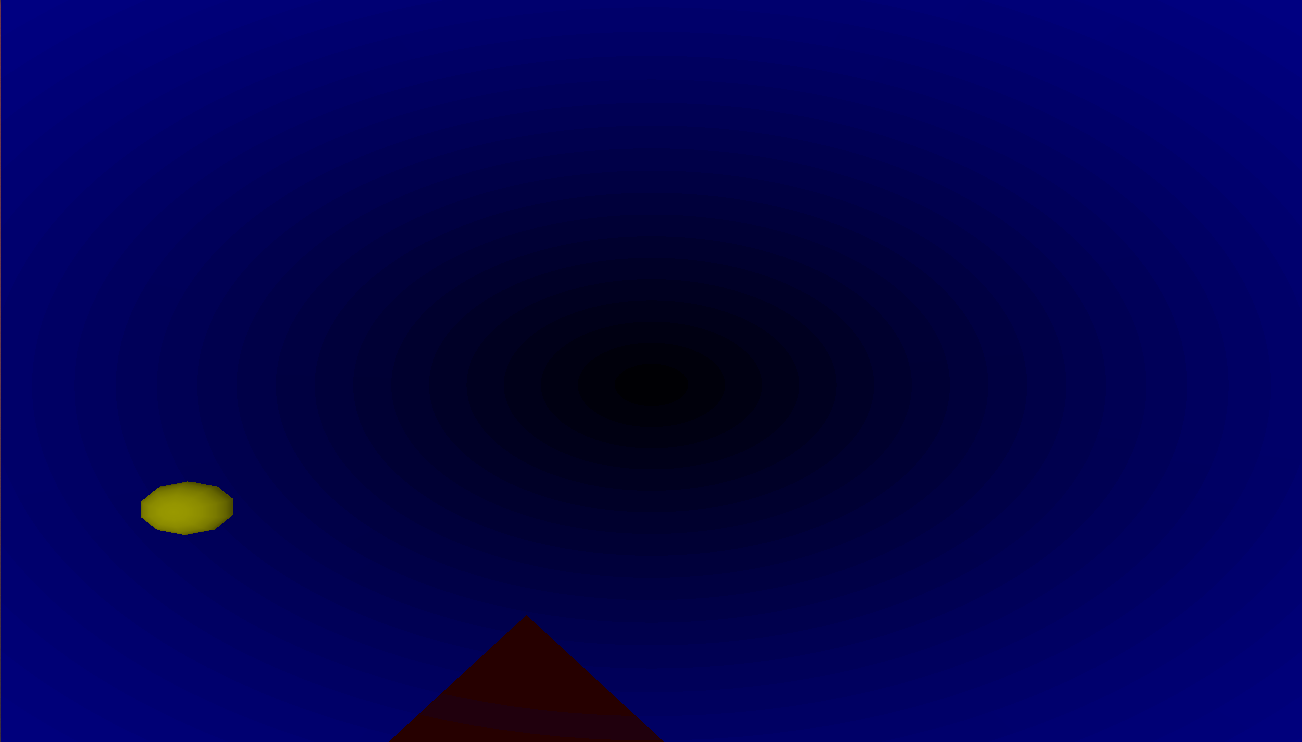
\includegraphics[width=1\linewidth]{lambert-screen.png}

Скриншот программы для зеркального отражения:

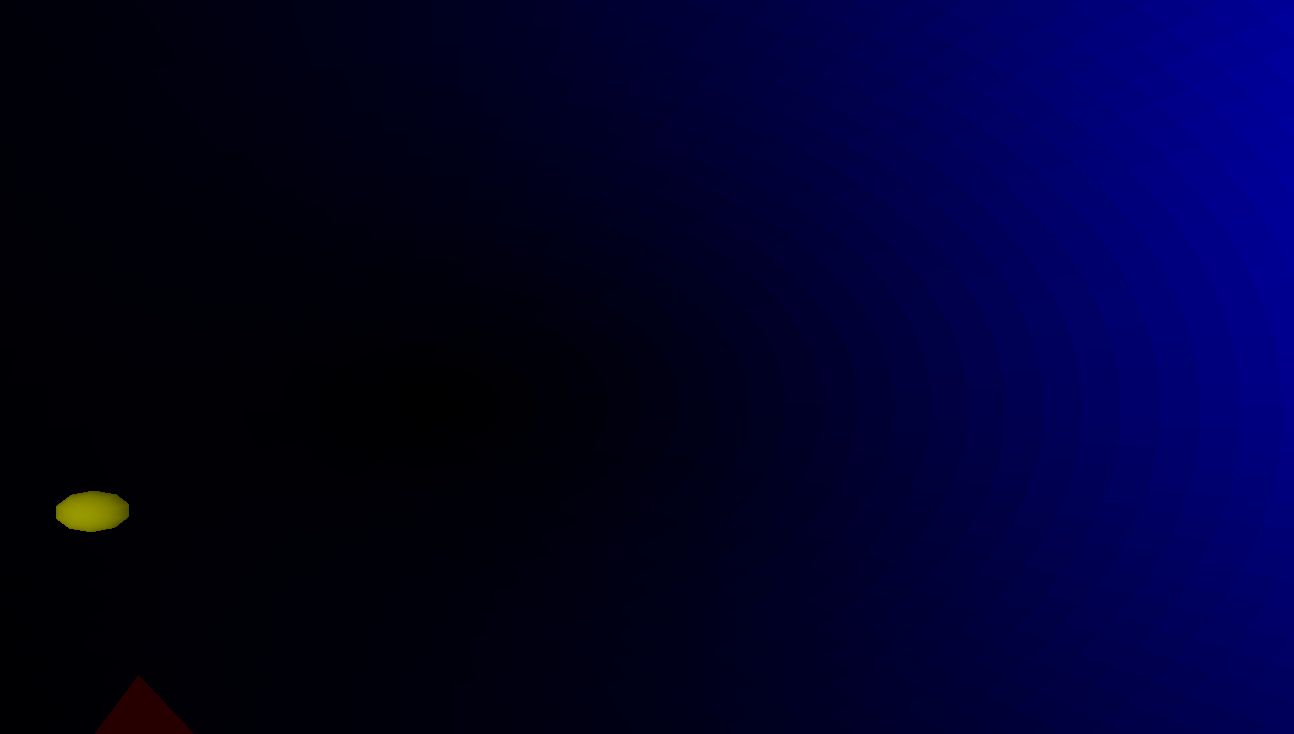
\includegraphics[width=1\linewidth]{zerkalo-screen.png}

Проекции сферы излучения (слева -- диффузное, справа -- зеркальное):

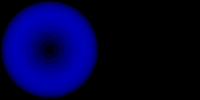
\includegraphics[width=0.499\linewidth]{lambert-map.png}
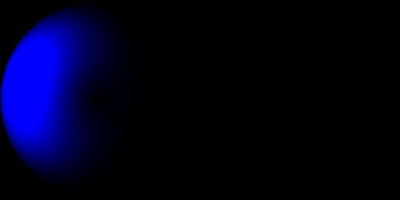
\includegraphics[width=0.499\linewidth]{zerkalo-map.png}

Таким образом, у нас есть возможность достаточно гибко моделировать различные материалы. 

\subsection*{Первичные и вторичные}

Рассмотрим одно положение объектов и сравним разницу между картинами в первом случае создаваемой только первично-освещенными областями и во втором -- совокупностью первичных и вторичных групп полигонов. 

Первично-освещенные области слева, вторичные -- справа:

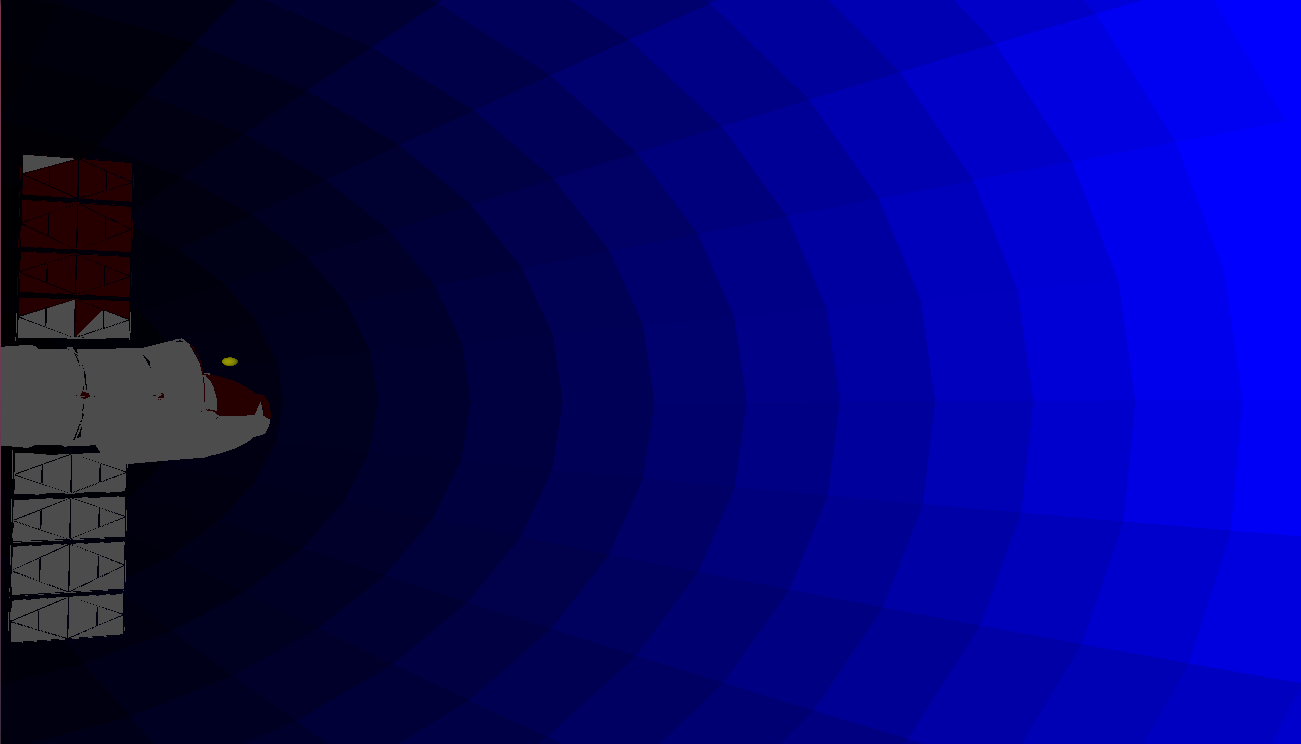
\includegraphics[width=0.499\linewidth]{first-screen-1.png}
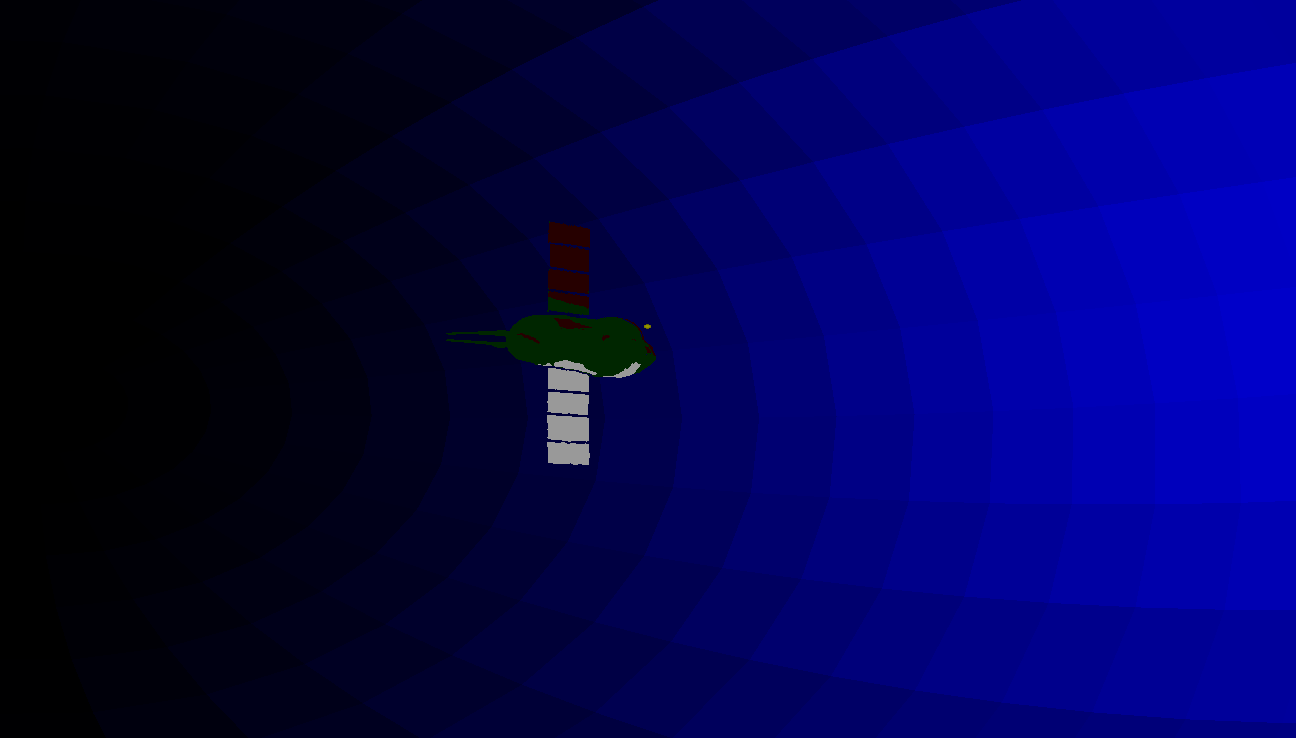
\includegraphics[width=0.499\linewidth]{second-screen-1.png}

Областью $A$ обозначено отражение от верхней антенной части корабля. Область $B$ -- пространство, излучение на карте проекций которого изменилось. 

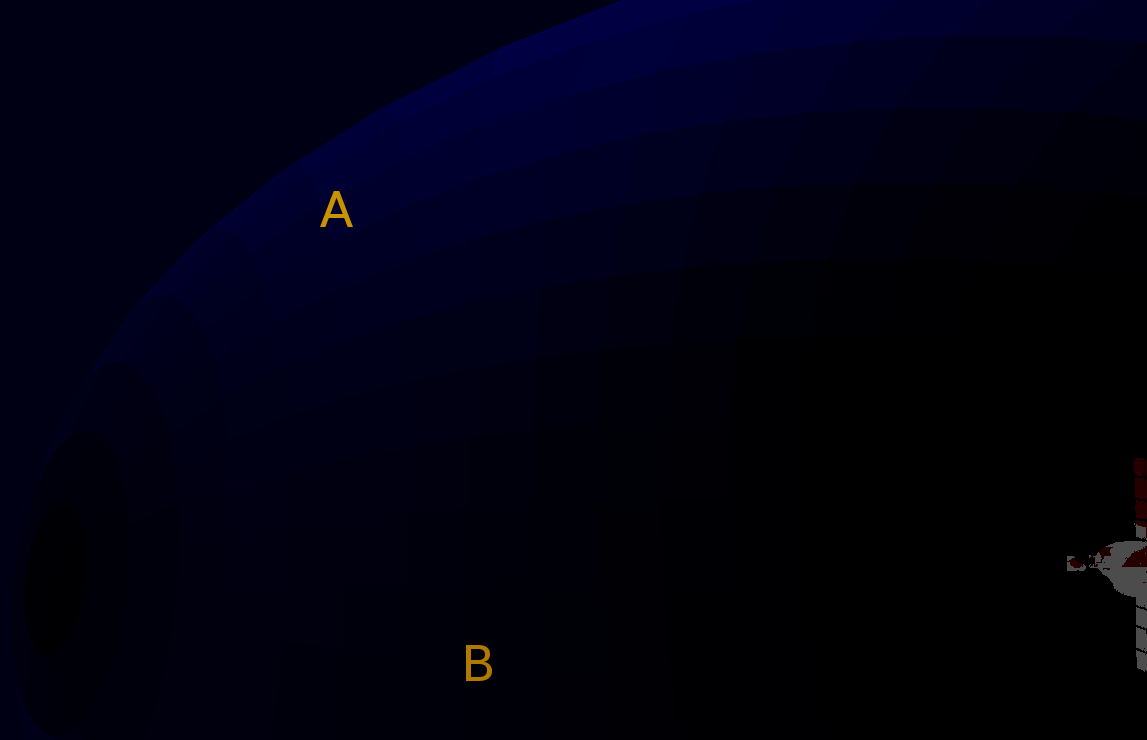
\includegraphics[width=0.51\linewidth]{first-screen-2.png}
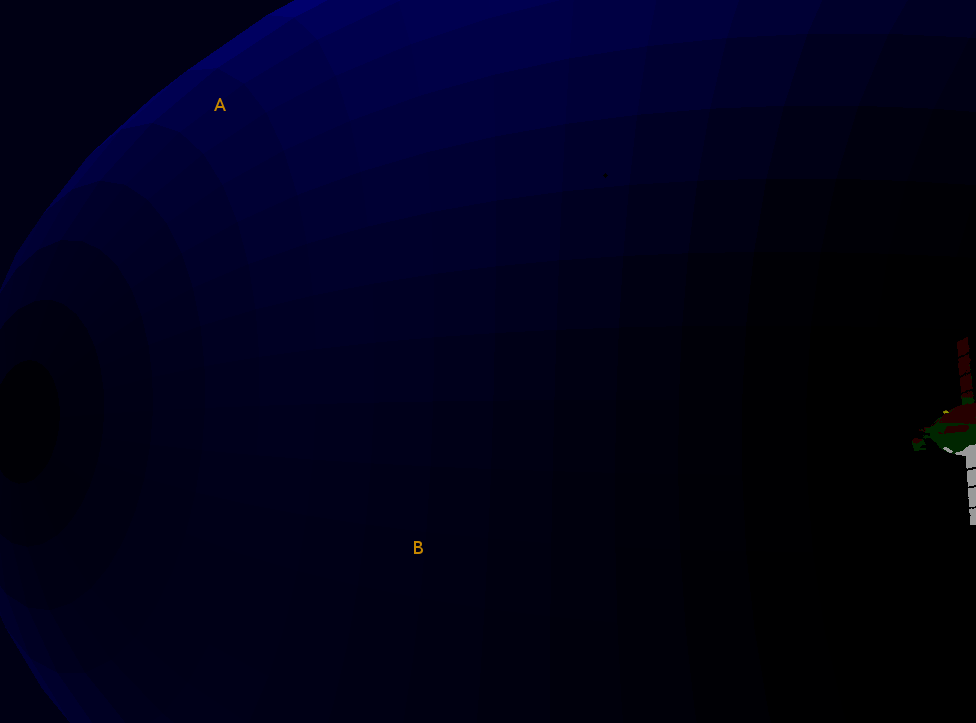
\includegraphics[width=0.445\linewidth]{second-screen-2.png}

Проекции сферы излучения (слева -- только первичные, справа первичные и вторичные области):

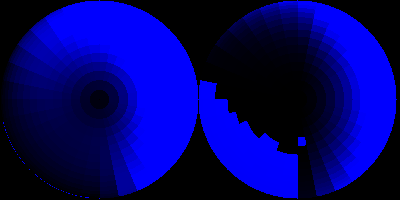
\includegraphics[width=0.499\linewidth]{first-map.png}
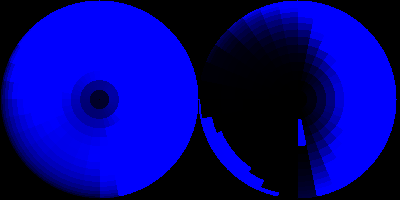
\includegraphics[width=0.499\linewidth]{second-map.png}

По картам заметно, левая нижняя область сферы (область $B$) стала светлее. Таким образом, в этой области существенный вклад вносит вторичное отражение. 

Таким образом, можно анализировать проекции сферы и выявлять области, в которых

1. излучение изменяется под влиянием вторичных зон (либо присутствует только переотраженный сигнал, либо присутствуют оба сигнала, но значения второго оказываются существенными),

2. излучение не подвергается изменениям (значение вторичного сигнала не существенно).

\subsection*{Сравнение производительности}

Проведем сравнение производительностей по моделированию поставленных нами задач. Помимо параллельной версии программы, запускаемой на графическом ускорителе, была написана последовательная версия программы, запускаемая на центральном процессоре.  

Характеристики центрального процессора (CPU): модель Intel Core 2 Duo T6600, тактовая частота 2200 MHz. 

Несмотря на то, что процессор многоядерный, программа была написана последовательно, то есть во время исполнении занято было только одно ядро.

Характеристики графического ускорителя (GPU): чипсет Nvidia GeForse GT 240M, объем 1024 mb.

Сравнение проводилось на трех сложных одинаковых полигональных моделях слонов с разной степенью детализации. Задача на GPU запускалась на сетке 65535 x 512 нитей.

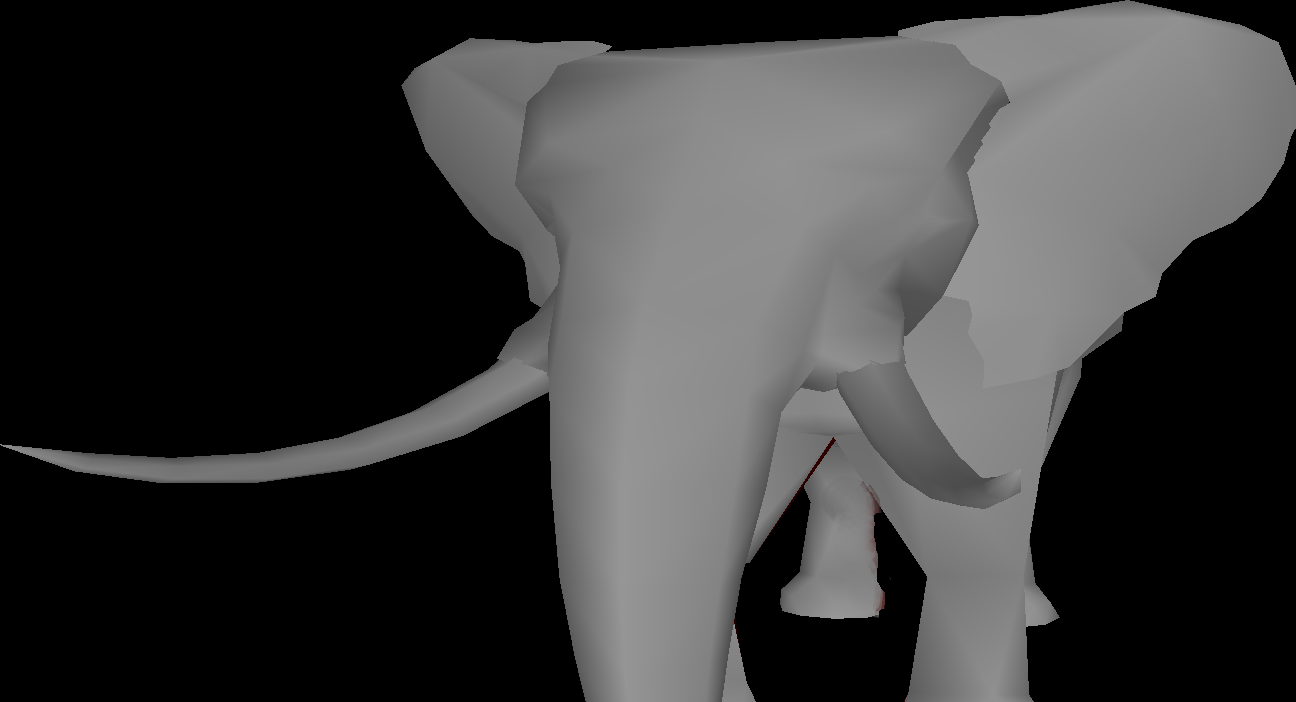
\includegraphics[width=0.28\linewidth]{elephav.png}
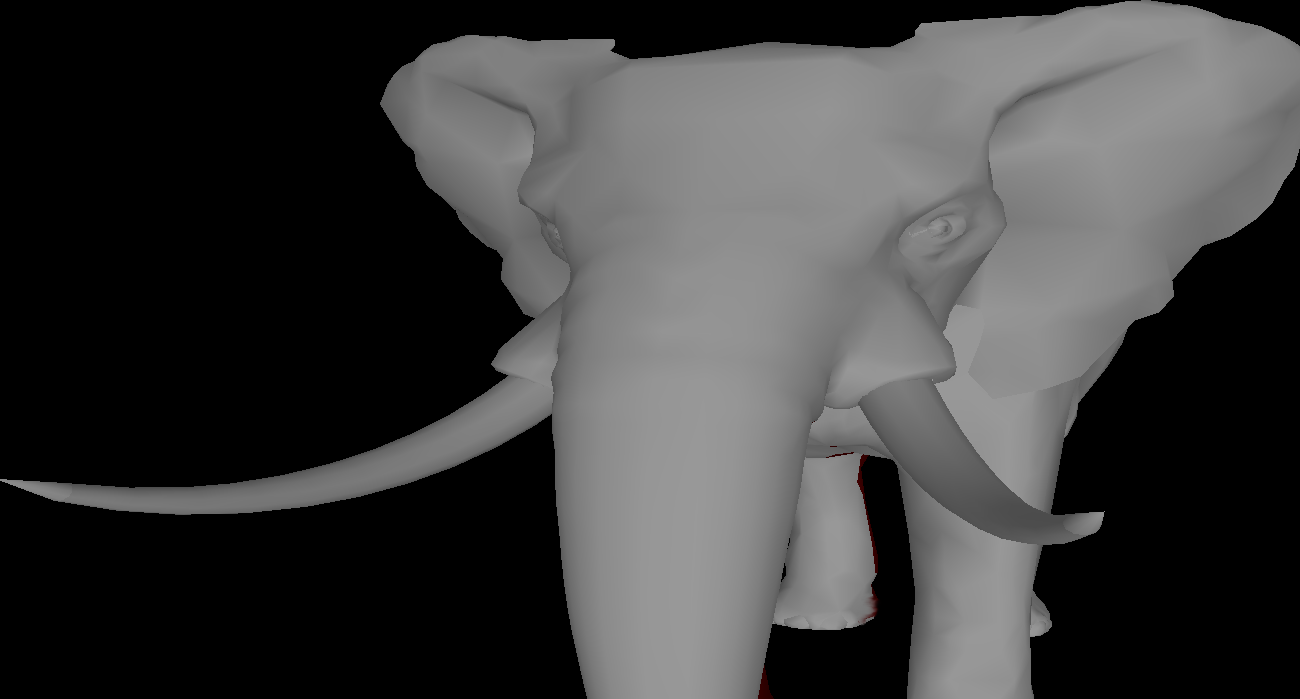
\includegraphics[width=0.28\linewidth]{elephal.png}
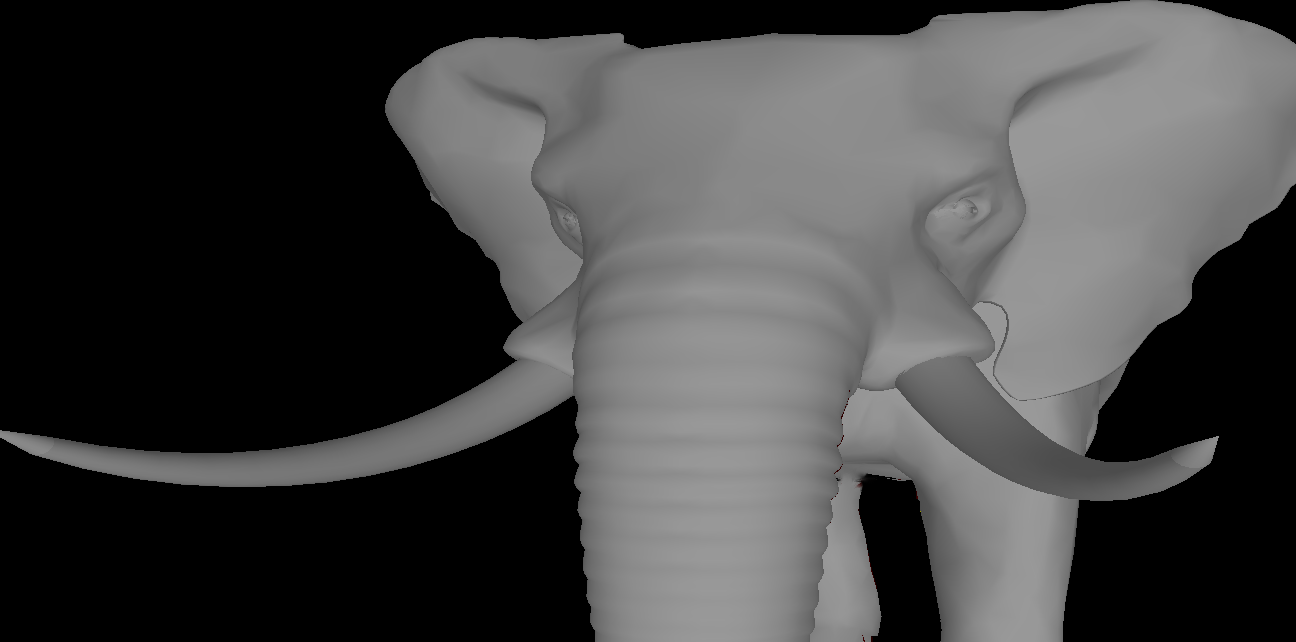
\includegraphics[width=0.305\linewidth]{elepham.png}

\begin{center}
Расчет первичных зон отражения
\begin{tabular}{cccc}
\textbf{время в мс}		& \textbf{слон 1148 гр} 			& \textbf{слон 10152 гр}		& \textbf{слон 39292 гр} 		\\
CPU 							& 172					 				& 16115								& 587850			 						\\
GPU 							& 105									& 	320								& 1292									\\
ускорение 					& 1.63								& 50.36								& 454.99 									\\
\end{tabular}
\end{center}

Таким образом, видно, что чем и крупнее задача, тем сильнее получаем ускорение. 




  \newpage
\begin{thebibliography}{99}

  \bibitem{sazonov}
  \textit{С.Б.\,Медведев, В.В.\,Сазонов, Х.У.\,Сайгираев}, Моделирование зон неустойчивой работы радиотехнической измерительной системы с активным ответом во время сближения и стыковки космических кораблей с Международной Космической Станцией
  // Математическое моделирование, 24(2):151–160, 2012.
  [\href{http://istina.imec.msu.ru/publications/article/533721/}{html}]

  \bibitem{soyz}
  Легедарный корабль <<Союз>>
  // Новости Космонавтики, апрель 2002


  \bibitem{boreskov1}
  \textit{А.В.\,Боресков, А.А.\,Харламов}, Основы работы с технологией CUDA
  // ДМК Пресс, 2010

  \bibitem{berezin}
  \textit{C.Б.\,Березин, В.М.\,Пасконов, Н.А.\,Сахарных}, Моделирование трехмерных течений методом расщепления с использованием параллельной архитектуры ГПУ
 // Вычислительные методы и программирование, 13: 75-81, 2012.
  [\href{http://num-meth.srcc.msu.ru/zhurnal/tom_2012/pdf/v13r210.pdf}{pdf}]

  \bibitem{cynami}
  \textit{М.А.\,Курако}, Оптимизация производительности вычислений для моделирования цунами на параллельных архитекутурах
  // Молодёжь и наука: Сборник материалов VII Всероссийской научно-технической конференции студентов, аспирантов и молодых учёных, посвященной 50-летию первого полета человека в космос
  [\href{http://elib.sfu-kras.ru/bitstream/2311/5869/1/s3_029.pdf}{pdf}]
  
  \bibitem{neuron}
  \textit{В.В.\,Парубец, О.Г.\,Берестнева, Д.В.\,Девятых}, Применение технологии CUDA для ускорения вычислений в нейронных сетях
  // Известия Томского политехнического университета, том 320, выпуск 5 (2012)

  \bibitem{radiolocation}
  \textit{П.В.\,Маковецкий, В.Г.\,Васильев}, Отражение радиолокационных сигналов -- лекции
  // Ленинградский институт авиационного приборостроения, 1975

  \bibitem{gugens}
  Принцип Гюйгенса-Френеля
  // Большая советская энциклопедия (3-е издание)

  \bibitem{ferma}
  \textit{Schuster A.}, An Introduction to the Theory of Optics. 
  //London: Edward Arnold (1904), 340 p.


  \bibitem{frenel}
  \textit{Hecht E.}, Optics. 
  //Addison Wesley, 1987. 457 p.


  \bibitem{lambert}
  \textit{Frank Pedrotti, Leno Pedrotti}, Introduction to Optics. 
  // Prentice Hall, 1993. ISBN 0135015456.  

  \bibitem{rendering-equ}
  \textit{J.\,Kajiya}, The rendering equation
  // ACM SIGGRAPH Computer Graphics, 1986. 20. N 4. P. 143-150

  \bibitem{history}
  \textit{Андрей Лебедев}, История развития алгоритмов глобального освещения
  // Компьютерная графика и мультимедиа, 2011
  [\href{http://cgm.computergraphics.ru/issues/issue19/globalillum}
  {html}]

  \bibitem{ray-tracing}
  \textit{Cook R., Porter T., Carpenter L.}, Distributed ray tracing
  // SIGGRAPH Comput. Graph, 1984. 18. N 3. P. 137-145.

  \bibitem{geometry}
  \textit{Moller T., Trumbore B.}, Fast, Minimum Storage Ray-Triangle Intersection 
  // J. Graphics Tools, 1997, v.2(1), p.21 -- 28.

  \bibitem{brezenhem}
  \textit{Роджерс Д.}, Алгоритмические основы машинной графики
  //Мир, 1989. — С. 512.

  \bibitem{3dda}, Анализ алгоритмов трассировки лучей для реалистичной визуализации трехмерных сцен и способов уменьшения их вычислительной сложности. 

  \textit{И.А. Запорожченко, М.А. Григорьев, С.А. Зори}, 
  //Цифровая обработка сигналов и изображений. – с. 353.
\end{thebibliography}


\end{document}
